\documentclass[a4paper,10pt]{article}

\usepackage[hidelinks]{hyperref}
\renewcommand{\figureautorefname}{Figura}
\renewcommand{\subsectionautorefname}{Sottosezione}
\usepackage{float}
\usepackage{tabularx}

% Lingua 
\usepackage[utf8]{inputenc}
\usepackage[italian]{babel}

% Margini
\usepackage{geometry}
\geometry{a4paper, top=3cm, bottom=3cm, left=3cm, right=3cm}
\setlength{\parindent}{0pt}

\usepackage{graphicx}   % per immagini
\usepackage{caption}    % per didascalie
\captionsetup[table]{labelformat=empty}
\usepackage{ifthen}     % per \ifthenelse
\usepackage{longtable}

\usepackage{array}      % per tabelle
\newcolumntype{M}[1]{>{\centering\arraybackslash}m{#1}}

\usepackage{datetime}

% Definisci un formato personalizzato
\newdateformat{italianformat}{\THEDAY~\monthname[\THEMONTH]~\THEYEAR}
\newdate{dataverbale}{04}{04}{2026}

% Definizione del formato con le barre
\newdateformat{slashdate}{\twodigit{\THEDAY}/\twodigit{\THEMONTH}/\THEYEAR}

% Per logo in ogni pagina
\usepackage{eso-pic}
\usepackage{tikz}
\AddToShipoutPictureBG{%
  \ifthenelse{\value{page}>1}{%
    \begin{tikzpicture}[remember picture, overlay]
      % Icona
      \node[anchor=north west, inner sep=0pt] at ([xshift=28pt,yshift=-28pt]current page.north west) 
        {
\includegraphics[width=1cm, height=1cm]{resources/Tool-8_icon_white.png}};
      
      % Riga
      \draw[black, line width=0.5pt] ([xshift=28pt + 1cm, yshift=-28pt - 0.6cm]current page.north west) 
            -- ++(3.2cm, 0);
      % Testo
      \node[anchor=west, text=black, font=\small] at ([xshift=28pt + 1cm, yshift=-28pt - 0.4cm]current page.north west) 
        {Specifica Tecnica};
    \end{tikzpicture}
  }{}
}

% Nome indice figure
\addto\captionsitalian{%
  \renewcommand{\listfigurename}{Indice delle immagini}%
}

\usepackage{listings}
\usepackage{xcolor}

\lstset{
    backgroundcolor=\color{gray!15},
    basicstyle=\ttfamily\small,
    frame=single,
    breaklines=true
}

%------Ridefinizione maketitle-------
\makeatletter
\renewcommand{\maketitle}{%
  \vspace*{\fill}
  \begin{center}
    {\LARGE \bfseries \@title \par}
    \vskip 1em
    {\large \@author \par}
    \vskip 1em
    {\large\slashdate{\displaydate{dataverbale}} \par}
  \end{center}
  \vspace*{\fill}
}
\makeatother
%-----------------------------------

\title{%
  
\includegraphics[width=10cm]{resources/Tool-8_white_2.png} \\[1.5ex]
  \textbf{\LARGE Manuale Utente}
}
\author{}
\date{\dataverbale}
\begin{document}
\tikz[remember picture,overlay] \node[opacity=0.2,inner sep=0pt] at (current page.center){
\includegraphics[width=\paperwidth,height=\paperheight]{resources/Abstract_lines.png}};

\maketitle

\newpage

\section*{Revisioni}
\begin{table}[h!]
\centering
\begin{tabular}{|M{0.8cm}|p{2.2cm}|p{5.7cm}|M{1.8cm}|p{2.2cm}|}
  \hline
  \textbf{Ver.} & \textbf{Autore} & \textbf{Modifiche} & \textbf{Data} & \textbf{Verifica} \\
    \hline
  0.3 & Besnik Murtezan & Stesura sezioni 3.4 , 3.5 , 4.1 & 06/05/2026 & - \\
  \hline
  0.2 & Giuliano Banchieri & Stesura parziale sezione "Istruzioni all'uso", stesura sottosezioni "Visualizzazione archivio note" e "Menù contestuale" & 30/04/2026 & Stefano Maso \\
  \hline
  0.1 & Stefano Maso & Prima stesura: struttura del documento e introduzione & 04/04/2026 & Niccolò Feltrin \\
  \hline
\end{tabular}
\caption{}
\label{tab:revisioni}
\end{table}

\newpage

\tableofcontents

\newpage

\listoffigures

\newpage

\section{Introduzione}
\subsection{Scopo del documento}
Il presente documento ha lo scopo di fornire un supporto completo agli utenti del sistema Second Brain, richiesto dall'azienda Zucchetti. Vengono dunque illustrate le istruzioni per l'utilizzo delle funzionalità fornite dall'applicazione oltre che i requisiti minimi necessari per il corretto funzionamento di Second Brain. \\
Eventuali termini tecnici sono definiti all'interno del documento "Glossario".

\subsection{Scopo del prodotto}
Il prodotto finale propone di realizzare un software che permetta la scrittura di testo con marcatori in formato MarkDown, la sua visualizzazione formattata correttamente e l’interazione con un LLM. In particolare, l’utilizzo di LLM verrà sfruttato da Second Brain per fornire funzionalità di riassunto, riscrittura, traduzione e generazione di testo in aggiunta ad una forma di critica secondo il modello dei ”Sei Cappelli per Pensare” di Edward De Bono. 

\subsection{Riferimenti}
\subsubsection{Riferimenti normativi}
\begin{enumerate}
    \item Capitolato C6 - Progetto Second Brain: \\ \url{https://www.math.unipd.it/~tullio/IS-1/2025/Progetto/C6.pdf}
    \item Regolamento progetto didattico: \\ \url{https://www.math.unipd.it/~tullio/IS-1/2025/Dispense/PD1.pdf}
    \item Norme di Progetto v1.1
\end{enumerate}
\subsubsection{Riferimenti informativi}
\begin{enumerate}
    \item \href{https://tool-8.github.io/Documentazione-SWE/glossario/Glossario.pdf}{Glossario v1.0} 
\end{enumerate}

\section{Requisiti per utilizzare il sistema}
Per il corretto utilizzo dell'applicazione è necessario soddisfare i seguenti requisiti minimi, i quali sono diversificati in base alla versione del prodotto che si intende utilizzare. 

\begin{table}[H]
\centering
\renewcommand{\arraystretch}{1.3}
\begin{tabular}{|l|l|}
\hline
\textbf{Sistema operativo} & \textbf{Distribuzione} \\ \hline

Linux & Ubuntu 22.04 LTS \\ 
Linux & Debian 12 \\ 
Linux & Fedora 39 \\ 

Windows & Windows 10 (WSL2) \\ 
Windows & Windows 11 \\ 

macOS & macOS 11 Big Sur \\ 
macOS & macOS 12 Monterey \\ \hline

\end{tabular}
\caption{Sistemi operativi supportati}
\end{table}

\begin{table}[H]
\centering
\renewcommand{\arraystretch}{1.3}
\begin{tabular}{|l|l|l|}
\hline
\textbf{Software} & \textbf{Versione} & \textbf{Download} \\ \hline
Docker & v29.0.1 & \href{https://www.docker.com}{docker.com} \\ 
& & \small (Consultato: 04/04/2026) \\ \hline
Makefile & v4.3 & \href{https://www.gnu.org/software/make/}{Sito Ufficiale GNU Make} \\ \hline


\end{tabular}
\caption{Software necessari}
\end{table}

\subsection{Requisiti hardware}
\begin{table}[H]
\centering
\renewcommand{\arraystretch}{1.3}
\begin{tabular}{|l|l|}
\hline
\textbf{Componente} & \textbf{Requisito minimo} \\ \hline

CPU & Dual-core 2.0 GHz \\ 
RAM & 4 GB \\ 
Storage & 10 GB disponibili \\ 
Rete & Connessione internet stabile \\ \hline

\end{tabular}
\caption{Requisiti hardware minimi}
\end{table}

\subsection{Requisiti software}
\begin{table}[H]
\centering
\renewcommand{\arraystretch}{1.3}
\begin{tabular}{|l|l|}
\hline
\textbf{Browser} & \textbf{Versione minima} \\ \hline

Google Chrome & 100+ \\ 
Mozilla Firefox & 100+ \\ 
Microsoft Edge & 100+ \\ 
Safari & 15+ \\ \hline

\end{tabular}
\caption{Requisiti software - Browser supportati}
\end{table}

\section{Istruzioni per l'installazione}
In questa sezione vengono fornite le istruzioni per l'installazione del prodotto software "Second Brain". Si consiglia di seguire attentamente i passaggi descritti per garantire un'installazione corretta.

\subsection{Clonazione repository}
È possibile ottenere una copia del progetto "Second Brain" attraverso due metodi principali:
\begin{enumerate}
  \item \textbf{Clonazione tramite Git:}
  
  Se si dispone di Git installato, è possibile clonare il repository ufficiale del progetto utilizzando il seguente comando nel terminale:

  \begin{lstlisting}
    git clone https://github.com/Tool-8/SecondBrain.git
  \end{lstlisting}
  \item \textbf{Download diretto:}
  
  In alternativa, è possibile scaricare direttamente il file ZIP del repository dal seguente link:

  \begin{center}
    \url{https://github.com/Tool-8/SecondBrain}
  \end{center}

  Dopo aver scaricato il file ZIP, è necessario estrarlo in una directory a scelta sul proprio computer.

\end{enumerate}

\subsection{Ottenimento chiavi API}
Per utilizzare le funzionalità di interazione con LLM, è necessario ottenere una chiave API.

Il nostro team ha scelto di utilizzare LLM gestite dall'azienda Zucchetti, pertanto è necessario accordarsi con essa per ottenere le chiavi API necessarie.

\subsection{Configurazione ambiente}
All'interno della cartella "src" è necessario creare un file di configurazione ".env".
\begin{enumerate}
  \item Aprire un terminale e spostarsi nella directory "src" del progetto.
  
  \begin{lstlisting}
    cd path/to/SecondBrain/src
  \end{lstlisting}

  \item Creare un file ".env" e inserire al suo interno il seguente contenuto:
  
  \begin{lstlisting}
    APP_NAME=SecondBrain
    APP_ENV=local
    APP_KEY=<TUA_CHIAVE_APP_KEY>
    APP_DEBUG=true
    APP_URL=http://localhost:8080

    APP_LOCALE=en
    APP_FALLBACK_LOCALE=en
    APP_FAKER_LOCALE=en_US

    APP_MAINTENANCE_DRIVER=file
    # APP_MAINTENANCE_STORE=database

    # PHP_CLI_SERVER_WORKERS=4

    BCRYPT_ROUNDS=12

    LOG_CHANNEL=stack
    LOG_STACK=single
    LOG_DEPRECATIONS_CHANNEL=null
    LOG_LEVEL=debug

    DB_CONNECTION=pgsql
    DB_HOST=db
    DB_PORT=5432
    DB_DATABASE=secondbrain
    DB_USERNAME=secondbrain
    DB_PASSWORD=secret

    SESSION_DRIVER=file
    SESSION_LIFETIME=120
    SESSION_ENCRYPT=false
    SESSION_PATH=/
    SESSION_DOMAIN=null

    BROADCAST_CONNECTION=log
    FILESYSTEM_DISK=local
    QUEUE_CONNECTION=sync

    CACHE_STORE=file
    # CACHE_PREFIX=

    MEMCACHED_HOST=127.0.0.1

    REDIS_CLIENT=phpredis
    REDIS_HOST=127.0.0.1
    REDIS_PASSWORD=null
    REDIS_PORT=6379

    MAIL_MAILER=log
    MAIL_SCHEME=null
    MAIL_HOST=127.0.0.1
    MAIL_PORT=2525
    MAIL_USERNAME=null
    MAIL_PASSWORD=null
    MAIL_FROM_ADDRESS="hello@example.com"
    MAIL_FROM_NAME="${APP_NAME}"

    AWS_ACCESS_KEY_ID=
    AWS_SECRET_ACCESS_KEY=
    AWS_DEFAULT_REGION=us-east-1
    AWS_BUCKET=
    AWS_USE_PATH_STYLE_ENDPOINT=false

    VITE_APP_NAME="${APP_NAME}"
    VITE_DEV_SERVER_URL=http://localhost:5173

    LLM_BASE_URL=<URL_BASE_LLM>
    LLM_API_KEY=<TUA_CHIAVE_API_KEY>
    # Modelli ['qwen3:30b','devstral:24b','gpt-oss:20b','gemma3:27b','gemma3:1b','deepseek-r1:8b','qwen3:1.7b']
    LLM_MODEL=gemma3:4b
  \end{lstlisting}

  \item Sostituire i valori di \verb|<URL_BASE_LLM>| e \verb|<TUA_CHIAVE_API_KEY>| con quelli ottenuti da Zucchetti.
  
  \begin{lstlisting}
    LLM_BASE_URL=<URL_BASE_LLM>      
    LLM_API_KEY=<TUA_CHIAVE_API_KEY>
  \end{lstlisting}
\end{enumerate}

\subsection{Installazione Dipendenze}
  All'interno della cartella "SecondBrain" è necessario eseguire il processo di installazione delle dipendenze.

\begin{enumerate}

  \item Aprire un terminale e spostarsi all'interno della root del progetto: 
  \begin{lstlisting}
    cd path/to/SecondBrain
  \end{lstlisting}

  \item Eseguire il processo di build dell'applicazione con i seguenti comandi da eseguire in sequenza:

  \begin{lstlisting}
    make prod
    make composer-install
    make bash
      php artisan key:generate
      php artisan migrate
      exit
    make npm-install

    ------------------------------------------
      O in caso non sia disponibile Makefile
    ------------------------------------------
    
    DOCKER_UID=$(id -u) DOCKER_GID=$(id -g) docker compose -f docker-compose.yml -f docker-compose.prod.yml up -d --build

    DOCKER_UID=$(id -u) DOCKER_GID=$(id -g) docker compose -f docker-compose.yml -f docker-compose.prod.yml exec app composer install

    DOCKER_UID=$(id -u) DOCKER_GID=$(id -g) docker compose -f docker-compose.yml -f docker-compose.prod.yml exec app sh

      php artisan key:generate
      php artisan migrate
      exit

    DOCKER_UID=$(id -u) DOCKER_GID=$(id -g) docker compose -f docker-compose.yml -f docker-compose.prod.yml exec app npm install
  \end{lstlisting}

  \item L'applicazione viene avviata automaticamente al termine dell'installazione. In caso si voglia terminare è sufficiente eseguire il comando:
  
  \begin{lstlisting}
    make down
  \end{lstlisting}

\end{enumerate}

\subsection{Esecuzione Applicazione}
Dopo aver installato l'applicazione, l'esecuzione avviene nel seguente modo:
\begin{enumerate}
  \item Avviare l'applicazione con il comando:

    \begin{lstlisting}
      make prod    

    ------------------------------------------
      O in caso non sia disponibile Makefile
    ------------------------------------------
    
      DOCKER_UID=$(id -u) DOCKER_GID=$(id -g) docker compose -f docker-compose.yml -f docker-compose.prod.yml up -d --build
    \end{lstlisting}

    
  \item Accedere all'applicazione aprendo il proprio browser all'indirizzo: \href{http://localhost:8080}{http://localhost:8080}

  \item Per terminare eventualmente l'applicazione è sufficiente eseguire il comando:
  
  \begin{lstlisting}
    make down

  ------------------------------------------
    O in caso non sia disponibile Makefile
  ------------------------------------------
    
    DOCKER_UID=$(id -u) DOCKER_GID=$(id -g) docker compose -f docker-compose.yml -f docker-compose.prod.yml down
  \end{lstlisting}

\end{enumerate} 

\newpage

\section{Istruzioni all'uso}
Tramite Second Brain, l'utente ha la possibilità di:
\begin{itemize}
    \item Visualizzare l'archivio delle note salvate
    \item Creare nuove note in formato Markdown
    \item Visualizzare, modificare ed eliminare note esistenti
    \item Interagire con LLM per essere assistito nella scrittura di una nota
    \item Importare file Markdown esterni
    \item Esportare le proprie note in formato Markdown, PDF o HTML
\end{itemize}

\subsection{Visualizzazione archivio note}
All'apertura dell'applicazione l'utente viene accolto da una schermata che mostra l'archivio delle note

\begin{center}
  \begin{figure}[H]
    \centering
    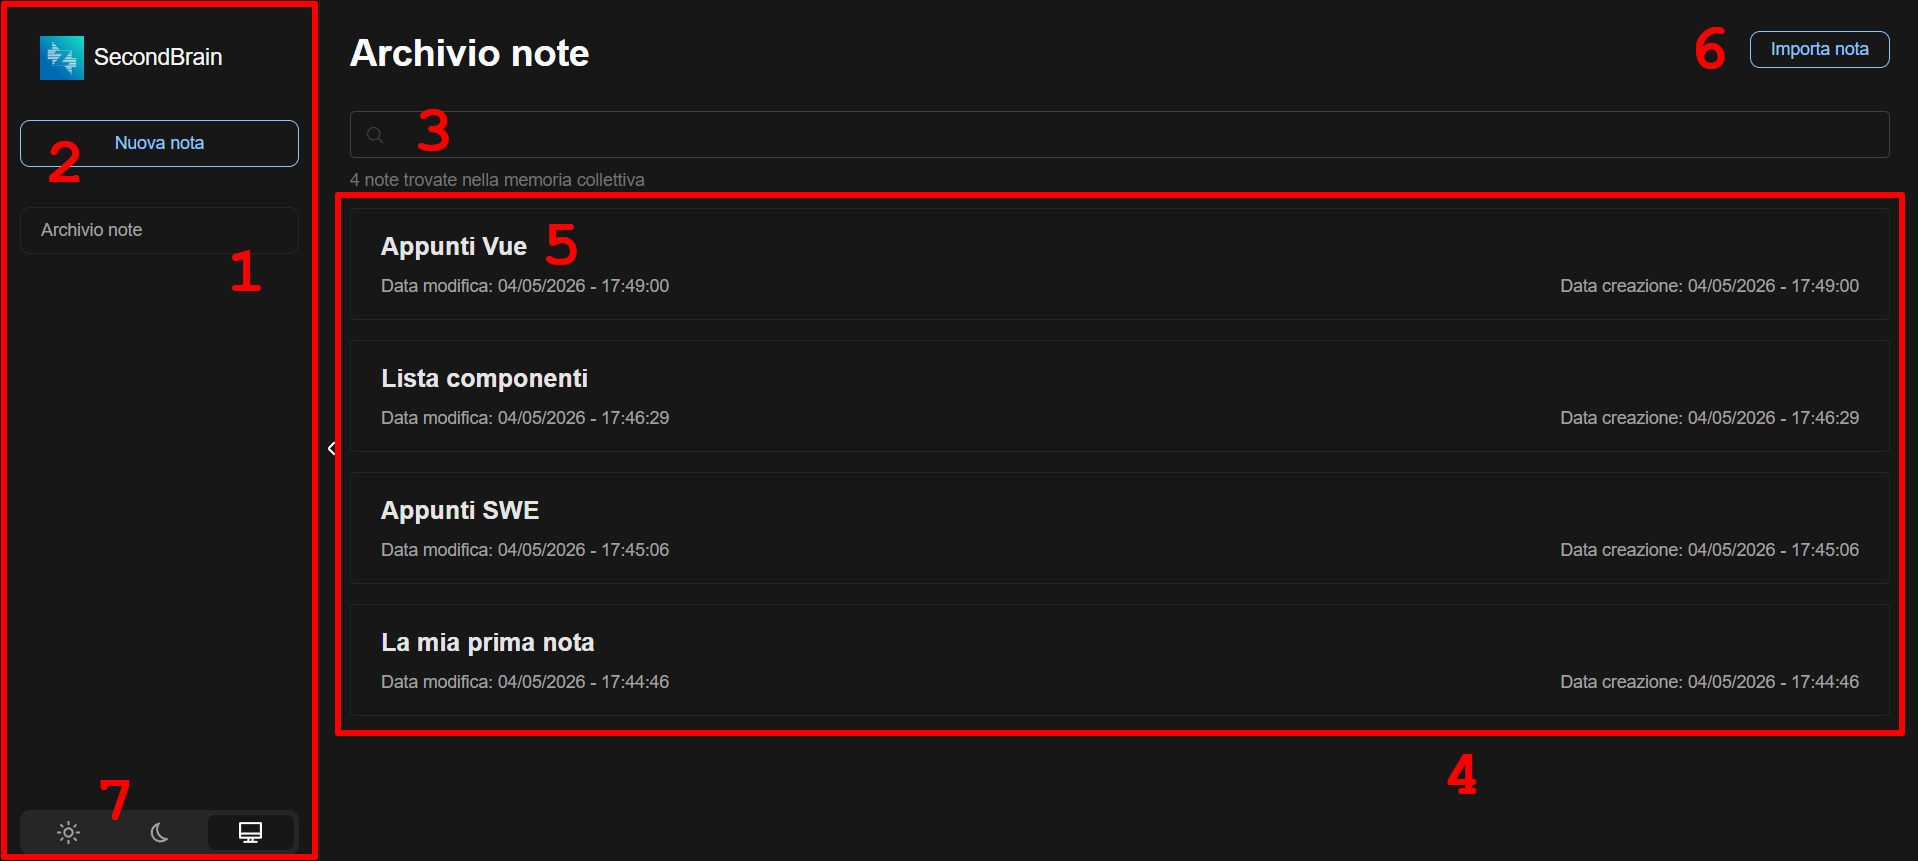
\includegraphics[width=1\textwidth]{resources/manual/archive/archivio.png}
    \caption{Schermata archivio note}
    \label{fig:archivio_note}
  \end{figure}
\end{center}

Questa schermata contiene:
\begin{enumerate}
  \item \textbf{Sidebar:} Permette all'utente di navigare fra le varie sezioni dell'applicazione, può essere nascosta o mostrata cliccando sulla freccia presente a sinistra.
  \item \textbf{Pulsante "Nuova nota":} Permette all'utente di creare una nuova nota in formato Markdown.
  \item \textbf{Barra di ricerca:} Permette all'utente di cercare una nota specifica all'interno dell'archivio, filtrando i risultati in tempo reale.
  \item \textbf{Elenco note:} Mostra tutte le note salvate all'interno dell'archivio.
  \item \textbf{Nota singola:} Cliccando su una nota, è possibile visualizzarne il contenuto completo, modificarla o eliminarla.
  \item \textbf{Pulsante "Importa nota":} Permette all'utente di importare un file Markdown esterno, aggiungendolo all'archivio delle note.
  \item \textbf{Selettore tema:} Permette all'utente di selezionare il tema dell'applicazione tra: chiaro, scuro, sistema.
\end{enumerate}

\subsubsection{Creazione Note}
Per creare una nota nuova è sufficiente cliccare sul relativo bottone \fcolorbox{black}{cyan!50}{Nuova nota} presente all'interno della SideBar (elemento \#2 nella \autoref{fig:archivio_note}). In seguito verrà aperto l'Editor di note con contenuto vuoto. (vedere \autoref{subsec:editor_note} per istruzioni dettagliate sull'Editor)

\subsubsection{Importazione Note}
SecondBrain permette anche la creazione di una nota attraverso l'importazione di un file locale in formato MarkDown selezionato dall'utente. Per utilizzare tale funzione è sufficiente cliccare il relativo bottone \fcolorbox{black}{cyan!50}{Importa nota} (elemento \#6 nella \autoref{fig:archivio_note}) all'interno dell'archivio note. In seguito verrà aperta una finestra modale in cui selezionare il file desiderato:

\begin{center}
  \begin{figure}[H]
    \centering
    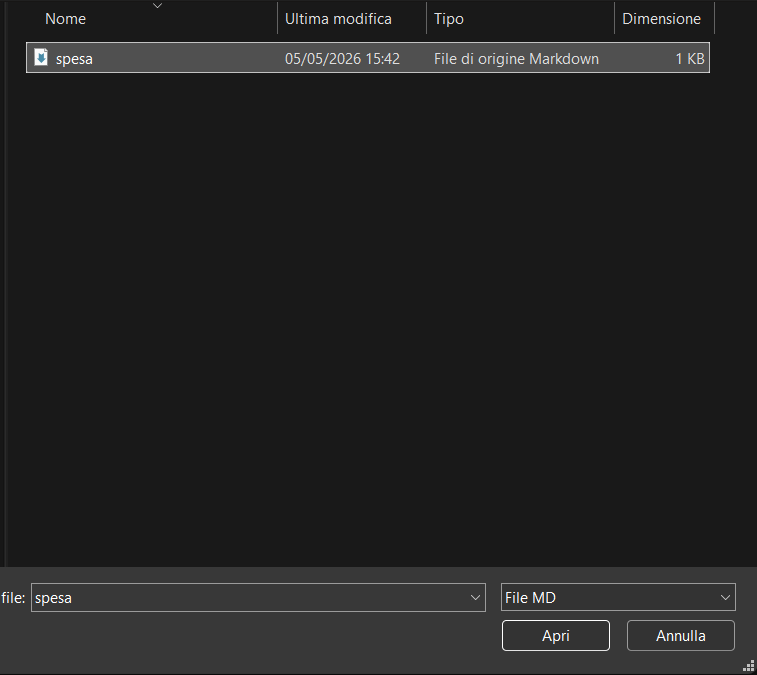
\includegraphics[width=0.45\textwidth]{resources/manual/archive/modale_import.png}
    \caption{Esempio finestra modale di selezione file (Windows 11)}
    \label{fig:modale_import}
  \end{figure}
\end{center}

Dopo aver selezionato il file e confermato l'azione il sistema provvederà ad effettuare l'importazione. Un avviso di successo notificherà l'utente dell'avvenuta creazione della nota nuova nell'archivio (il titolo è formato dal nome del file seguito dal dataora di importazione).

\begin{center}
  \begin{figure}[H]
    \centering
    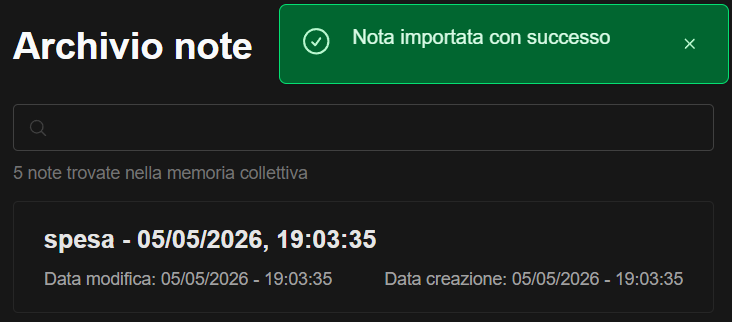
\includegraphics[width=0.4\textwidth]{resources/manual/archive/successo_import.png}
    \caption{Nota importata con relativo avviso di successo}
    \label{fig:successo_import}
  \end{figure}
\end{center}

Qualora si tentasse di importare un file con formato non supportato il sistema notificherà l'utente dell'errore senza proseguire ulteriormente con l'importazione:

\begin{center}
  \begin{figure}[H]
    \centering
    
\includegraphics[width=0.35\textwidth]{resources/manual/archive/errore_formato_import.png}
    \caption{Avviso di errore per formato non supportato}
    \label{fig:errore_formato_import}
  \end{figure}
\end{center}

\subsubsection{Apertura Note}
Cliccando con il tasto sx una delle note presenti nell'archivio si aprirà l'Editor di note; al suo interno è possibile visualizzare e modificare il contenuto della nota. (vedere \autoref{subsec:editor_note} per istruzioni dettagliate sull'Editor)

\subsubsection{Ricerca Note}
Per effettuare una ricerca delle note in base al nome è sufficiente inserire il termine nella casella di ricerca (elemento \#3 nella \autoref{fig:archivio_note}) e premere "Invio".
La lista delle note verrà aggiornata con i risultati della ricerca.

\begin{center}
  \begin{figure}[H]
    \centering
    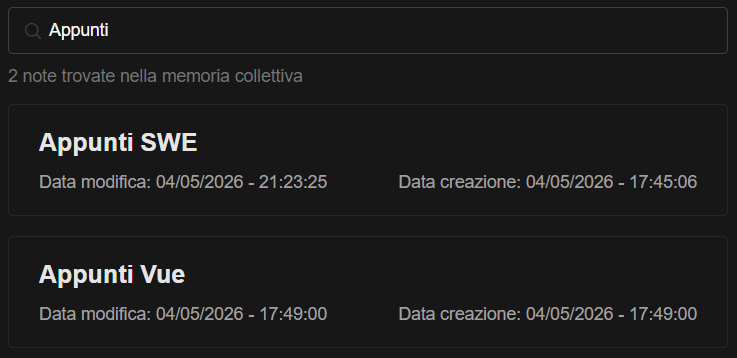
\includegraphics[width=0.6\textwidth]{resources/manual/archive/ricerca_archivio.png}
    \caption{Esempio di ricerca}
    \label{fig:ricerca_archivio}
  \end{figure}
\end{center}

\subsubsection{Azioni contestuali}
Cliccando con il tasto destro su una nota all'interno dell'archivio, è possibile accedere al seguente menu contestuale:

\begin{center}
  \begin{figure}[H]
    \centering
    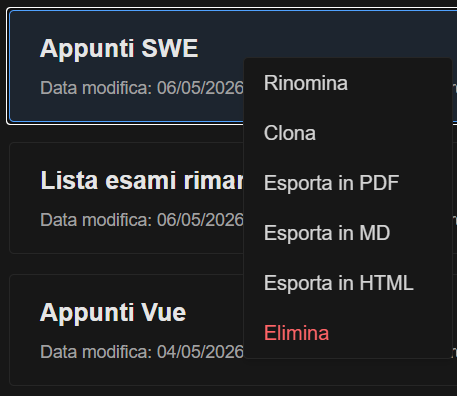
\includegraphics[width=0.4\textwidth]{resources/manual/archive/menu_context_nota_archivio.png}
    \caption{Menu contestuale nota in archivio}
    \label{fig:menu_contestuale}
  \end{figure}
\end{center}

Le azioni possibili sono le seguenti:

\clearpage

  \paragraph{\fcolorbox{black}{blue!15}{Rinominazione nota}}

    Cliccando sulla relativa opzione \fcolorbox{black}{cyan!50}{Rinomina} del menu contestuale (\autoref{fig:menu_contestuale}), l'utente può rinominare la nota selezionata attraverso la finestra modale visualizzata.
    
    \begin{center}
      \begin{figure}[H]
        \centering
        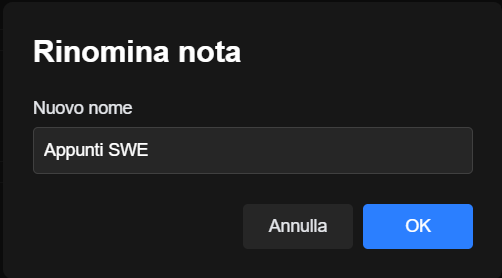
\includegraphics[width=0.4\textwidth]{resources/manual/archive/modale_rinomina_archivio.png}
        \caption{Finestra modale di rinominazione nota}
        \label{fig:modale_rinomina_archivio}
      \end{figure}
    \end{center}

    In seguito alla conferma da parte dell'utente viene effettuato un controllo di unicità del titolo: in caso di successo viene mostrato il relativo avviso di avvenuta rinominazione. 
    
    \begin{center}
      \begin{figure}[H]
        \centering
        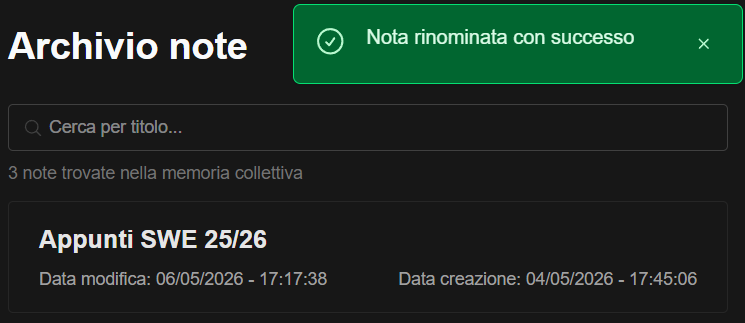
\includegraphics[width=0.5\textwidth]{resources/manual/archive/successo_rinomina_archivio.png}
        \caption{Nota rinominata con relativo avviso di successo}
        \label{fig:successo_rinomina_archivio}
      \end{figure}
    \end{center}

    In caso contrario viene visualizzato un messaggio di errore e la nota mantiene il titolo precedente.

    \begin{center}
      \begin{figure}[H]
        \centering
        
\includegraphics[width=0.35\textwidth]{resources/manual/archive/errore_titolo_rinomina_archivio.png}
        \caption{Avviso di errore titolo già in uso}
        \label{fig:errore_titolo_rinomina_archivio}
      \end{figure}
    \end{center}

  \paragraph{\fcolorbox{black}{blue!15}{Clonazione nota}}

    Cliccando sulla relativa opzione \fcolorbox{black}{cyan!50}{Clona} del menu contestuale (\autoref{fig:menu_contestuale}), l'utente può clonare la nota selezionata (creare una copia) attraverso la finestra modale visualizzata.
    Il sistema propone il titolo originale seguito dal dataora di clonazione come titolo per la nota clonata; l'utente può in ogni caso personalizzarlo. 

    \begin{center}
      \begin{figure}[H]
        \centering
        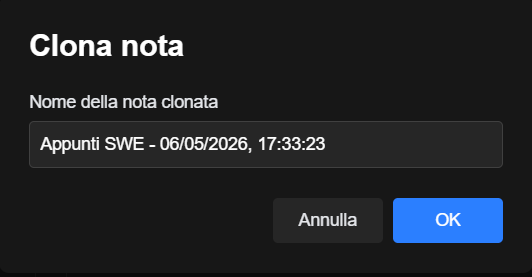
\includegraphics[width=0.4\textwidth]{resources/manual/archive/modale_clona_archivio.png}
        \caption{Finestra modale di clonazione nota}
        \label{fig:modale_clona_archivio}
      \end{figure}
    \end{center}

    Dopo la conferma il sistema effettua un controllo di unicità del titolo; in caso di successo viene mostrato il relativo avviso di avvenuta clonazione.
    
    \begin{center}
      \begin{figure}[H]
        \centering
        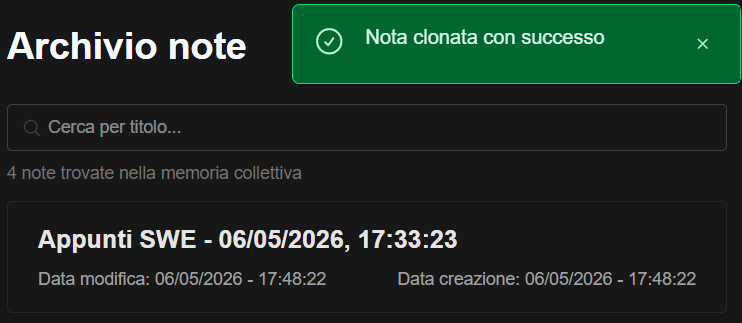
\includegraphics[width=0.5\textwidth]{resources/manual/archive/successo_clona_archivio.png}
        \caption{Nota clonata con relativo avviso di successo}
        \label{fig:successo_clona_archivio}
      \end{figure}

      In caso di titolo già utilizzato viene visualizzato un messaggio di errore (vedi \autoref{fig:errore_titolo_rinomina_archivio}).

    \end{center}

\vspace{2cm}

  \paragraph{\fcolorbox{black}{blue!15}{Esportazione nota}}

    L'utente può esportare una nota presente in archivio in uno dei seguenti formati:
        \begin{itemize}
          \item PDF
          \item Markdown
          \item HTML
        \end{itemize}
    Cliccando su una delle opzioni \fcolorbox{black}{cyan!50}{Esporta} del menu contestuale (\autoref{fig:menu_contestuale}), il sistema fornirà al browser un file nel formato selezionato; un avviso notificherà l'utente del successo dell'esportazione ed automaticamente verrà avviato il download del file.
    
    \begin{center}
      \begin{figure}[H]
        \centering
        
\includegraphics[width=0.4\textwidth]{resources/manual/archive/successo_esporta_archivio.png}
        \caption{Avviso di successo esportazione}
        \label{fig:successo_esportazione}
      \end{figure}

      \begin{figure}[H]
        \centering
        
\includegraphics[width=0.3\textwidth]{resources/manual/archive/esempio_download_esporta_pdf.png}
        
\includegraphics[width=0.3\textwidth]{resources/manual/archive/esempio_download_esporta_md.png}
        
\includegraphics[width=0.3\textwidth]{resources/manual/archive/esempio_download_esporta_html.png}
        \caption{Esempi di file generati dall'esportazione nei vari formati (Windows 11)}
        \label{fig:esempio_file_esportazione}
      \end{figure}
    \end{center}

  \clearpage

  \paragraph{\fcolorbox{black}{red!20}{Eliminazione nota}}

    Cliccando sulla relativa opzione \fcolorbox{black}{red!40}{Elimina} del menu contestuale (\autoref{fig:menu_contestuale}), l'utente può eliminare la nota selezionata. Viene mostrata una finestra modale di conferma:

    \begin{center}
      \begin{figure}[H]
        \centering
        
\includegraphics[width=0.5\textwidth]{resources/manual/archive/modale_elimina.png}
        \caption{Finestra modale di eliminazione nota}
        \label{fig:modale_elimina}
      \end{figure}
    \end{center}

    In caso si confermi l'azione, la nota verrà rimossa in modo definitivo e verrà visualizzato un messaggio di avvenuta eliminazione.

    \begin{center}
      \begin{figure}[H]
        \centering
        
\includegraphics[width=0.4\textwidth]{resources/manual/archive/successo_elimina.png}
        \caption{Avviso di avvenuta eliminazione}
        \label{fig:successo_elimina}
      \end{figure}
    \end{center}

\subsection{Editor Note}\label{subsec:editor_note}
Inizialmente vengono mostrate sia la sezione di testo compreso di sintassi Markdown (Editor), sia la sezione di testo formattato (Render).

\begin{center}
\huge{\textbf{\fbox{SEZIONE DA COMPLETARE}}}
\end{center}

\newpage

\section{Supporto tecnico}
Per assistenza tecnica relativa all'utilizzo del prodotto software "Second Brain", viene fornito il seguente indirizzo email: 
\begin{center}
    tool8eight@gmail.com
\end{center}
Per un servizio più efficiente, si è pregati di includere nel corpo dell'email una descrizione più completa possibile del problema riscontrato, insieme ad ogni possibile screenshot o dettaglio aggiuntivo che possano risultare utili alla risoluzione di quest'ultimo. \\
Si invita, inoltre, a descrivere eventuali passaggi già tentati per risolvere il problema, in modo che il gruppo possa fornire un'assistenza più mirata.
\end{document}

